
\section{Datafari}

\subsection{Installation}

Für Datafari musste folgende Software nachinstalliert werden: Java 8 und JQ. Es muss allerdings für Java die JAVA\_HOME-Variable erstellt werden. Insofern Datafari nicht unter Root laufen soll, muss noch ein besonderer Nutzer mit Root Rechten angelegt werden. Dieser muss wie schon bei Solr höhere User-Limits erhalten. Datafari installiert sich selbst durch eine DEB-Datei. Während der Installation erscheint ein Setup-Dialog, welcher einen durch die Konfiguration führt. Das Starten des Server geschieht als letztes durch ein Script in dem Installationsordner.

\subsection{Indexierung}

Um eine Indexierung durchzuführen muss bei Datafari eine sogenanntes Repository angelegt werden. In diesem werden die Datenbank-Verbindung eingetragen. Hierbei ist es wichtig, dass vorher der Treiber korrekt installiert wird. Hierbei kam es zu Problemen. Das auf Apache ManifoldCF basierende System akzeptiert nur MySQL-JDBC Treiber. Da der MariaDB-Treiber einen anderen Klassenpfad verwendet, funktioniert dieser nicht. \begin{quote} This connection type cannot be configured to work with other databases than the ones listed above without software changes.~\cite[S.~61]{ApacheSoftwareFoundation.}\end{quote} Deswegen habe ich für diesen Test den MySQL-Treiber von Oracle verwendet.
Nachdem der Treiber korrekt installiert ist und das Repository erstellt ist, kann man nun einen Job zu Indexierung der Einträge starten. In dem werden die Queries und der Zeitplan konfiguriert.


\subsection{Oberfläche}

Die Oberfläche von Datafari ist dreigeteilt. Zum einen ist dort, eine Such-Oberfläche, welche sich ohne Anmeldung erreichen lässt. Als zweites gibt es eine Administrationsoberfläche, welche erst eingesehen werden kann, sobald man eingeloggt ist. Dort findet man diverse Einstellungen für die Suchmaschinen, wie Synonyme oder die Facetten-Konfiguration. Auch sind dort die Logs einzusehen, was aber eigentlich nur eine Einbindung des ELK-Stacks ist. Die dritte Oberfläche ist die Einstellungsseite für die Datacrawler. Dies ist eine modifizierte Oberfläche von Apache ManifoldCF. Generell sind die einzelnen Menüs sehr übersichtlich gestaltet und haben leicht zu verstehende Titel.

\subsection{Dokumentation}

Die Dokumentation geht sehr genau auf die Installation des Systems ein, dabei werden alle Konfigurationsaspekte beleuchtet. Zum Beispiel wird beschrieben, wie die User Limits erhöht werden, oder die JAVA\_HOME-Variable korrekt gesetzt wird. Allerdings merkt man an manchen Stellen, dass die Dokumentation nicht von nativen Englischsprechende geschrieben wurde, da die Grammatik nicht immer stimmt. Allerdings hat dies nie zu Problemen oder Verwechslungen geführt.
Die Dokumentation zum Einrichten des JDBC-Treibers finden sich einige Probleme \ref{img:datafariJDBC}. Zum einen sind beide Pfade, die in dem Text angegeben sind, falsch. Einer davon wird sogar anders in dem Screenshot direkt darunter angezeigt. Und zum anderen ist der zweite Screenshot so niedrig aufgelöst, dass sich nicht viel erkennen lässt. Dies passiert auch, wenn das Bild in einen neuen Tab geladen wird. Generell ist die Dokumentation für den Umgang mit Datenbanken nicht sehr ausführlich. Die Erklärungen, wofür die Variables bei der Erstellung eines Jobs stehen, mussten in der Dokumentation von ManifoldCF nachgelesen werden.

\begin{figure}
	\centering
	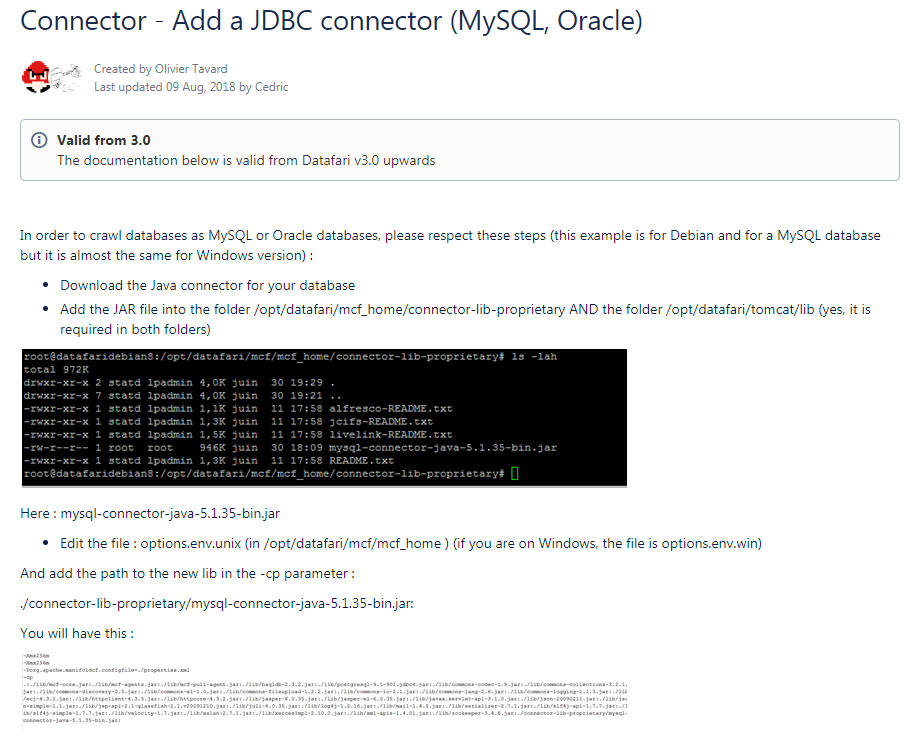
\includegraphics[width=1\linewidth]{images/datafari_doku_wrong_path.png}
	\caption{Dokumentationsseite für den JDBC Treibers von Datafari.}
	\label{img:datafariJDBC}
\end{figure}


\subsection{Absetzen einer Anfrage und Integration in PHP}
